\chapter{Projekt}

\section{Einführung}
Neben der fachlichen Auseinandersetzung mit dem Thema “gesunder Lebensstil”, haben wir ein Projekt durchgeführt.
\newline
In diesem Projekt wollen wir selbst erfahren, was wir für Veränderung, sowie Unterschiede bemerken, wenn wir gesund leben.
\newline
Die \textit{“Einschränkungen”} für ein gesunden Lebensstil, haben wir anhand, der vorherigen Kapiteln bestimmt. Zusätzlich haben wir versucht, diese möglichst alltagstauglich zu definieren. Auf die \textit{“Einschränkungen”} gehen wir später noch genauer ein.
\newline
Dieses Projekt haben wir insgesamt vier Wochen im Zeitraum vom \textit{21.10.2020} bis \textit{17.11.2020} durchgeführt.
\subsection{Vorheriger Lebensstil}
\subsubsection{Von Dario Grob}
Wie schon im Kapitel \ref{bezug:dario} angesprochen, habe ich über eine länger Zeit nicht auf einen gesunden Lebensstil geachtet. In den letzten Sommerferien haben ich beschlossen, mich regelmässiger sportlich zu betätigen und einen Schlafrhythmus zu etablieren.
\newline
In den Herbstferien bin ich jedoch in alte Muster zurückgefallen. Ein normaler Arbeitstag hat folgendermassen ausgesehen.
\newline
Ich gehe ca. um 02:45 Uhr ins Bett und muss um 08:15 Uhr aufstehen. Somit schlafe ich durschnittlich 5h 30min pro Nacht. Dadurch bin den ganzen Tag sehr müde und trinke viel Energydrinks und Kaffee um mich wach zu halten. 
\newline
Über den Mittag esse ich auswärts. Dies ist oft Fast Food und eher ungesund.
\newline
Bis um 18:30 Uhr arbeite ich und gehe daraufhin nach hause. Das Abendessen Zuhause ist oft gesund, da meine Mutter kocht und auf eine gesunde Ernährung achtet. 
\newline
In meiner Freizeit game ich sehr viel oder schaue Serien und bewege mich somit nicht viel. 
\newline
Die Hausaufgaben, das Lernen auf Tests, sowie das Arbeiten an Projekten schiebe ich solang es geht vor mir her. Dadurch bin ich vor den Schultagen sehr in stress.
\newline
Den ganzen Tag durch mache ich regelmässig Pausen und rauche dazu eine Zigarette oder nehme ein Snus. Durschnittlich rauche ich am Tag 10 Zigaretten und nehme 3 - 4 Snus.
\newline
Durch meinen Lebensstil habe ich negative folgen. Ich habe oft starke Rückenschmerzen durch das viele Sitzen und der fehlenden Bewegung, bin oft sehr müde dadurch, dass ich sehr wenig schlafe und nehme in letzter Zeit an Gewicht zu.
\subsubsection{Von Bastian Büeler}
Früher habe ich immer wenig geschlafen und bin ca. zwischen 24:00-02:00 Uhr schlafen gegangen. Weil ich zu wenig Nachtruhe hatte und mein Körper viel mehr Schlaf gebraucht hätte, war ich am Folgetag oftmals sehr müde. Ebenfalls habe ich immer wieder ungesundes Essen zu mir genommen, wie zum Beispiel Pizza. Zudem habe ich nicht auf die Ernährungspyramide geachtet und einfach irgendwie gegessen. Dazu kam noch die Müdigkeit, welche zusätzlich hungrig machte. Die Aufgaben habe ich mir im Kopf gemerkt und keine ToDo Liste oder sonstiges erstellt und die Bewegung hat seit der Corona Krise ebenfalls stark abgenommen. Alles in allem würde ich sagen, dass mein vorheriger Lebensstil nicht wirklich gesund war.
\subsubsection{Von Jonas Schultheiss}
Ich habe dieses Thema schon in Kapitel \ref{bezug:jonas} angesprochen.
\newline
Mitte bis Ende der Sekundarschule habe ich mich etwas gehen lassen. Dies betrifft das ganze Spektrum von Aspekten, in welchen es in unserer Vertiefungsarbeit geht. Sport, Schlaf und so weiter. Nachdem ich es im Unihockeyverein nicht in die U18A geschaft habe, hatte ich keine Lust mehr auf Unihockey. Denn mir blieb nur die Wahl in einen deutlich schlechteren Verein zu wechseln, wo ich niemanden kannte und einen längeren Weg hätte, oder aufzuhören. Dannach machte ich eine Pause vom Sport, bis ich ein Jahr später mit Volleyball in Therwil begann. Dies zog ich zwei Jahre durch, bis ich schlussendlich aufhörte, wegen meiner Körpergrösse (173cm) und weil ich mich meiner Meinung nach zu langsam verbesserte. Ein halbes Jahr später gab ich Unihockey nochmals eine Chance. Ein paar meiner Kollegen sind in einem Verein in Flüh und nahmen mich mit. Ich spielte für ein Semester, bis aufhörte. Ich hatte sehr Probleme mitzuhalten, da ich mit 16 die grandiose Idee hatte, mit dem rauchen anzufangen. In meinem alten Verein war ich noch einer der Besten, wenn es um die Ausdauer ging. Meine Position auf dem Feld war sogar die, die am meisten Aussdauer benötigte. Nun, 3 Jahre später konnte ich nun nur noch zehn Minuten voll mitspielen, bevor meine Lunge zu schmerzen began und ich mich am liebsten übergäben hätte.
\newline
Wie schon angesprochen habe ich im Januar 2017 angefangen zu rauchen. Vor dem Begin der Lehre habe ich zwei Monate lang aufgehört und dachte mir, ich würde nie wieder rauchen. Anfangs der Sommerferien hatte ich allerdings einen \textit{sehr} schlechten Tag, worrauf hin ich wieder began. Seither habe ich unzählige Male probiert aufzuhören. Doch habe es bisher nie komplett geschaft. Nach zwei Tagen habe ich extreme Konzentrationsprobleme und werde durch Kleinigkeiten sehr aggressiv. Da diese zwei Aspekte in der Berufsschule oder im Betrieb eher störend sind, habe ich es immer auf die Ferien gelegt. Die Situation mit der Lunge in verbindung mit Sport brachte mich zum Umstieg von Zigarette zu Snus. Ich denke nicht, dass Snus im Allgemeinen weniger schädlich ist, doch ich kann nun aus Erfahrung sagen, dass sich meine Lunge regeneriert hat. Ich kann nun wieder relativ Problemlos joggen gehen.
\newline
Nun würde ich gerne zu meinem Konsum von koffeinhaltigen Getränken kommen. Während beziehungsweise nach meinen extremen Schlafproblemen ist dieser Konsum geradezu explodiert. Zuvor habe ich an manchen Tagen 250ml zu mir genommen. Doch während und nachdem ist es meist an jedem Tag die gleiche bis die dreifache Menge. Ich war am morgen komplett unbrauchbar ohne das Koffein, weil ich während den Problemen oft nur drei bis sechs Stunden schlief. Dann konnte ich das Problem mit Schlaftabletten in den Griff bekommen. Durch diese konnte ich zwar einschlafen, doch war am Morgen genau so müde wie zuvor. Mittlerweile nehme ich die Tabletten nicht mehr. Doch aus dieser Phase ist nun eine Gewohnheit geworden. Trinke ich mal nicht eines, fühle ich mich unkonzentriert und müde, obwohl ich genug geschlafen habe. Ich fühle mich nicht so müde wie während dem Problem, sondern ich spüre einfach, dass mir etwas fehlt.
\pagebreak
\subsection{Was machen wir?}
\subsubsection{Ernährung}
In unserem Projekt achten wir auf unser Ernährung. Dabei richten wir uns nach der Definition aus dem Kapitel “Ernährung”.
\newline
Unser Ernährung dokumentieren wir in der App “Lifesum”. In dieser App sind “alle” Lebensmittel und Nahrungsmittel hinterlegt. Dazu liefert die App eine kurze Zusammenfassung, ob ein Nahrungsmittel gesund ist und was für Inhaltsstoffe dies hat. Neben dem Dokumentieren unserer Ernährung, konnten wir uns an Rezeptvorschläge der App orientieren, falls wir etwas kochen mussten.
\newline
\begin{figure}[!ht]
  \centering
  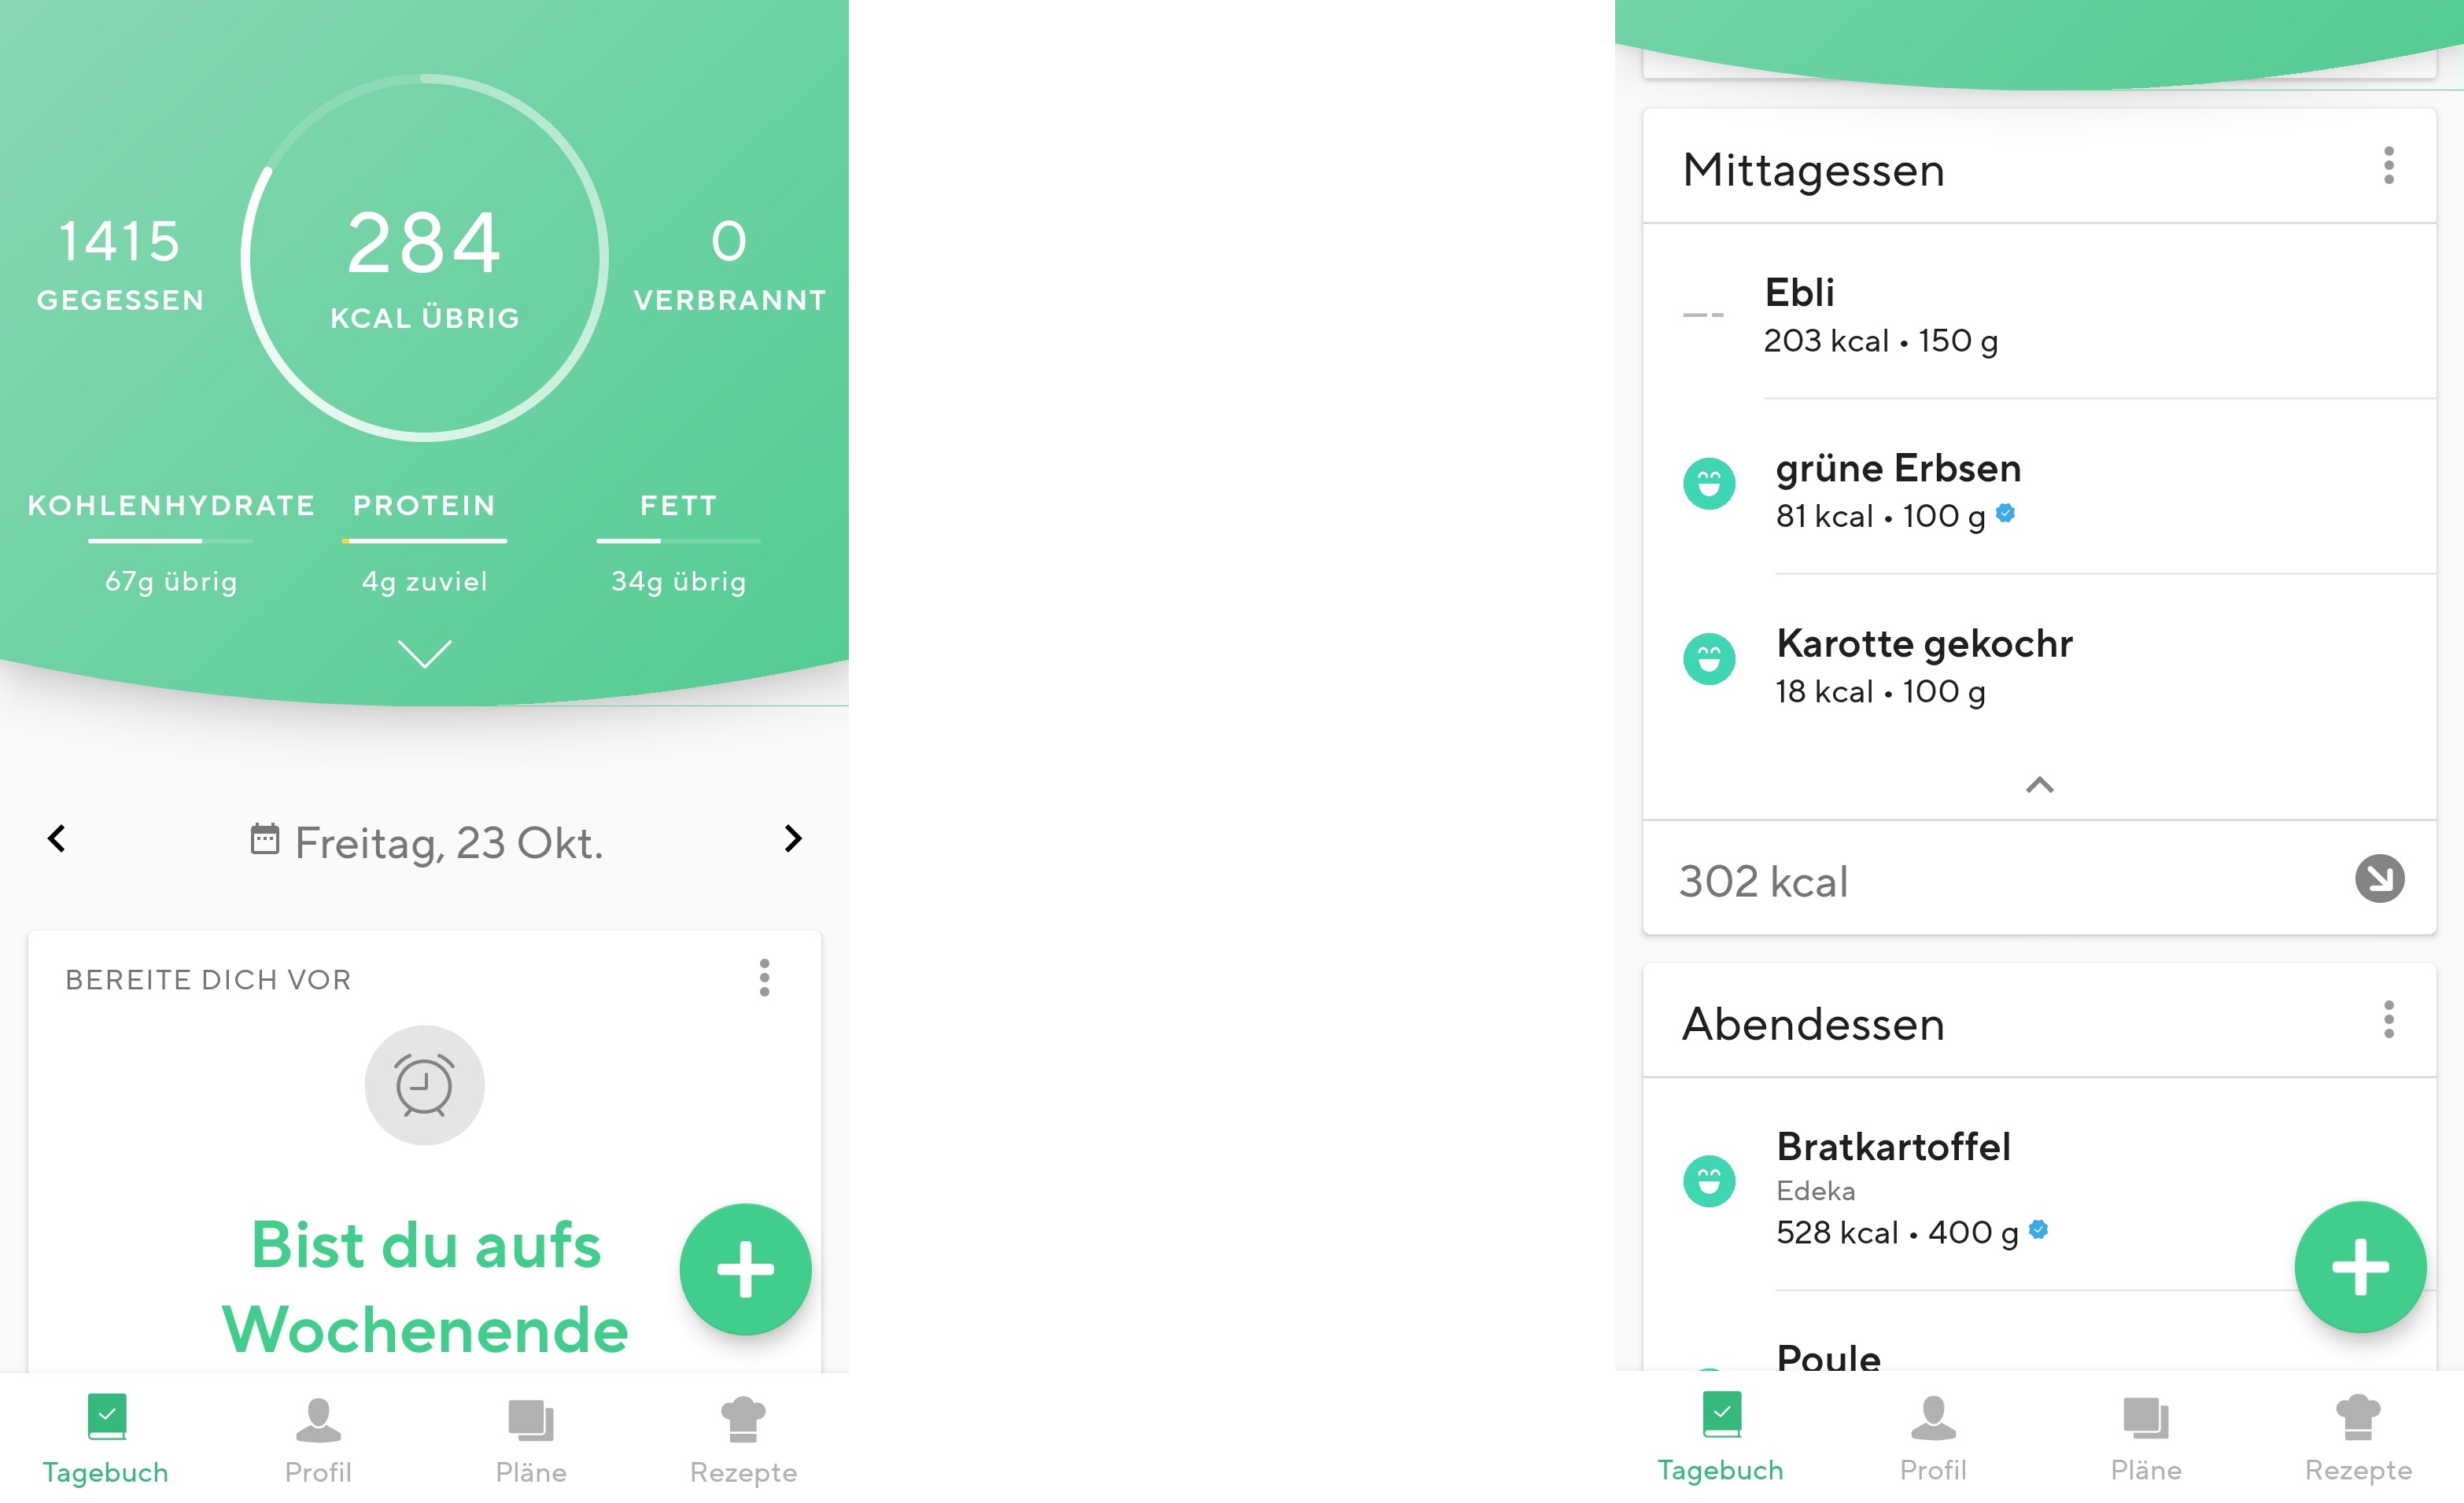
\includegraphics[width=0.7\linewidth]{./images/app.png}
  \caption{Screenshots der App “Lifesum”}
  \label{fig:app_1}
\end{figure}
\newline
\begin{figure}[!ht]
  \centering
  \includegraphics[width=0.7\linewidth]{./images/food.png}
  \caption{Beispiele einer Mahlzeit}
  \label{fig:app_1}
\end{figure}
\newline
\subsubsection{Bewegung}
Zu einem gesunden Lebensstil gehört auch eine gewisse Bewegung, damit wir fit bleiben. Dies haben wir auch in unserem Projekt berücksichtigt und umgesetzt. Unsere Punkte bezüglich der Bewegung waren: Regelmässigkeit, Strukturierung, sowie Abwechslung. Mit diesen Punkten sind wir herangegangen und haben uns einen Plan aufgestellt, was wir machen wollen und in welchen Abständen wir die Übungen durchführen wollen. Somit haben wir eine Strukturierung und eine Regelmässigkeit in das Ganze hereingebracht. Für die Abwechslung haben wir uns entschieden auf verschiedene Arten zu trainieren, damit wir insgesamt nicht nur zum Beispiel die Muskulatur trainieren, sondern auch die Ausdauer. Dafür haben wir einen Plan zusammengestellt, welchen wir jede Woche durchführen werden. Diesen kann man in der folgenden Tabelle anschauen:
\newline
\newline
\textbf{Bewegungs- / Fitnessplan}
\newline
\begin{table}[htp]
  \begin{tabularx}{\textwidth}{l X}\hline \\
    \textbf{Tag} & \textbf{Übung}  \\\hline \\
    1 & \textbf{Pull, Legs:} Rücken, Beine, Bizeps, Sixpack \\
    2 & Keine -> Pause \\
    3 & \textbf{Push:} Brust, Schulter, Trizeps, Sixpack \\
    4 & Keine -> Pause \\
    5 & \textbf{Ausdauer:} HIIT + Joggen/Seilspringen \\
    6 & Keine -> Pause \\
    7 & Keine -> Pause \\
    \\\hline
  \end{tabularx}
\end{table}
\newline
Die Übungen haben wir von einem Youtuber namens Sascha Huber, welcher ein Spezialist im Bereich Fitness und Ernährung ist. Ebenfalls haben wir ein HIIT Workout von der Youtuberin Pamela Reif, welche ebenfalls sehr bekannt für ihre Kenntnisse im Sport und Ernährungsbereich ist. Bei den Übungen haben wir uns vor allem darauf fokussiert, dass sie möglichst alltagstauglich sind und man nicht viel Vorahnung dafür braucht. Deswegen wird in den Videos entweder mit dem Körpergewicht oder mit Kurzhanteln gearbeitet. Die Auswahl der Videos belief sich darauf, dass wir praktisch alle Trainingsvideos von Sascha Huber nahmen. Der Grund dafür war, dass er die Übungen am Besten erklärte sowie vorzeigte. Auch kam man schnell zurecht und das volle Bewegungsprogramm wurde abgedeckt.
\newline
\pagebreak
\newline
\textbf{Genauer Bewegungs- und Fitnessplan}
\newline
\begin{table}[htp]
  \begin{tabularx}{\textwidth}{l X}\hline \\
    \textbf{Muskelgruppe} & \textbf{Links}  \\\hline \\
    Pull, Legs, Sixpack & \url{https://m.youtube.com/watch?v=B1qXC1qlzcA}
    \newline
    \url{https://m.youtube.com/watch?v=vwLV2sCSQEo}
    \newline
    \url{https://m.youtube.com/watch?v=bcH-qcnpy20}
    \newline
    \url{https://m.youtube.com/watch?v=8Tdk6k3TBpk}
    \newline
    \url{https://m.youtube.com/watch?v=iBHhj6AQ75I} \\ \\
    Push, Sixpack & \url{https://m.youtube.com/watch?v=B1qXC1qlzcA}
    \newline
    \url{https://m.youtube.com/watch?v=HnU27M-7NXU}
    \newline
    \url{https://m.youtube.com/watch?v=4JZxm_qJPUc}
    \newline
    \url{https://m.youtube.com/watch?v=-QRYwdtDpGI}
    \newline
    \url{https://m.youtube.com/watch?v=iBHhj6AQ75I} \\ \\
    Ausdauer & \url{https://youtu.be/V0PtkzDVI5U}
    \newline
    oder
    \newline
    \url{https://youtu.be/06cwQlikBEA}
    \newline
    danach entweder Joggen (x)min oder Seilspringen (x)min \\
    \\\hline
  \end{tabularx}
\end{table}
\subsubsection{Schlaf}
Wir haben die Unterthemen des Mindmaps in Bezug auf Schlaf genommen und dazu einige Regeln aufgestellt, welche wir während unseres Projekt stets befolgen mussten. 
\newline
Auf dem Mindmap haben wir folgende Punkte aufgezeigt: Qualität, Rhythmus, feste Ruhezeit und elektrische Ruhezeit. 
\newline
\newline
Unsere Umsetzung der einzelnen Themen war wie folgt:
\begin{itemize}
  \item \textbf{Qualität}
  \newline
  Um die Qualität des Schlafs zu verbessern haben wir eine Regel aufgestellt, dass man nur im Bett ist um zu schlafen. Sonstige Aktivitäten, wie zum Beispiel Entspannen, Unterhaltungsmedien anschauen und sonstige werden an anderen Orten getätigt. Der Grund dieser Regel ist die Wertschätzung und Einzigartigkeit des Bettes. Laut der Uni Münster ist dies sehr wichtig, damit der Körper nichts durcheinander bringt. Er weiss durch diese Regel genau, dass das Bett nur zum Schlafen ist. Dies wird alles von unserem Unterbewusstsein dementsprechend wahrgenommen. 
  \item \textbf{Rhythmus}
  \newline
  Ein fester Schlafrhythmus ist sehr wichtig für unseren Körper. Laut der Uni Münster erleichtert es den Körper sich auf feste Zeiten einzustellen und stärkt die innere Uhr. Dies hat zur Folge, dass der Körper weiss, wann es Zeit ist ins Bett zu gehen und wann man wieder aufwachen sollte. Wir hatten uns ebenfalls einen Rhythmus gesetzt. Dieser war individuell, jedoch war er abhängig von der festen Ruhezeit, welche mindestens 7h und 30min entsprach.
  \item \textbf{Feste Ruhezeit}
  \newline
  Unsere Umsetzung der festen Ruhezeit entsprach einer festen Zeit welche wir definierten. Wir haben uns dabei nicht auf feste “Bettzeiten” und “Aufstehzeiten” geeinigt sondern jeglich auf einen festen Wert, welchen man pro Nacht mindestens schlafen muss. Unsere feste Ruhezeit waren demnach mindestens 7 Stunden und 30 Minuten pro Nacht. Alles über dieser Zeit ist gut, unter diese sollte man jedoch nicht fallen. 
  \item \textbf{Elektrische Ruhezeit}
  \newline
  Als elektrische Ruhezeit definierten wir 30 Minuten. Diese Zeit ist direkt vor dem Schlafen und dient zur Entspannung des Körpers. Wir wollten damit unseren Körper vor dem Blaulicht von den elektrischen Geräten schützen, damit wir einen besseren Schlaf haben und besser einschlafen können. Diese Zeit war aber nicht in die feste Ruhezeit von 7h und 30min miteinbezogen, sondern wurde darauf gerechnet. Dadurch waren wir bei einer Ruhezeit von 8h, sowie einer Schlafenszeit von mindestens 7h und 30min.
\end{itemize}
\subsubsection{Zeitmanagement}
Auch auf das Zeitmanagement möchten wir in unserem Projekt eingehen. Die Methode 'Bullet Journaling' wird in Kapitel \ref{bulletjournaling} genau beschrieben. Wir werden folgende Methoden Anwenden:
\newline
\begin{table}[htp]
  \begin{tabularx}{\textwidth}{l X}\hline \\
    \textbf{Kandidat} & \textbf{Angewandte Methode}  \\\hline \\
    \textbf{Dario Grob} & ToDo Liste \\
    \textbf{Bastian Büeler} & ToDo Liste \\
    \textbf{Jonas Schultheiss} & Bullet Journaling und White Board
    \\\hline
  \end{tabularx}
\end{table}
\newline
Das verwenden dieser Methoden sollte unseren Stress veringern und uns unter anderem bei der Erstellung dieser Vertiefungsarbeit helfen. Dario und Bastian haben sich die Bullet Journaling Methode angesehen. Für sie ist es allerdings nicht den Auwand wert, daher machen sie ToDo-Listen mit dem Smartphone. Dies reicht vollkommen aus. Da ich schon seit dem Frühling Bullet Journaling betreibt, wird er dies so weiterführen.
\subsubsection{Gewohnheiten}
Wir versuchen in unserem Projekt “schlechte” Gewohnheiten möglichst zu vermeiden und “gute” Gewohnheiten zu etablieren. Dabei legen wir den Fokus auf die Gewohnheiten, welche wir in Kapitel “Gewohnheiten” angeschaut haben.
\newline
Da es sehr schwer ist mit schlechten Gewohnheiten, wie zum Beispiel dem Rauchen, verbieten wir diese nicht ganz. Das Ziel ist es ein besseres Bewusstsein für diese Gewohnheiten zu erhalten und die Regelmässigkeit zu minimieren.
\subsubsection{Bullet Journaling}
\label{bulletjournaling}
Das Dokumentieren der Vergangenheit, organisieren der Gegenwart und die vorbereitung auf die Zukunft.
\newline
Dies Klingt nach einer Herausforderung, die uns allen bekannt vorkommt.
\newline
Ryder Carroll, ein in New York lebender Designer, machte sich mit seinem Notizbuch auf den Weg, dieses Problem frontal anzugehen. Vor etwa acht Jahren entwickelte Ryder das Bullet Journal, ein analoges System, das als ToDo-Liste, Tagebuch, Notizbuch und Skizzenbuch konzipiert war. Dabei konzipierte er vier Aspekte, welche das Grundgerüst des Bullet Journals bilden \cite{bulletjournal_2020} :
\begin{itemize}
  \item \textbf{Rapid logging} - Ein System, mit dem sich sehr schnell Notizen machen lassen, indem Seitenzahlen, Titel und verschiedene Aufzählungszeichen verwendet, um Schritte, die bei Aufgaben unternommen werden müssen, zu unterscheiden.
  \item \textbf{Module} - Erlauben es, die Notizen, die gemacht werden, auf verschiedene Weise zu organisieren. Am Anfang gibt es eine Seite, auf der die Titel für alle Einträge hinzugefügt werden, damit später schnell darauf zurückgegriffen werden kann.
  \item \textbf{Monthly log} - Ein Kalender und eine monatliche ToDo-Liste.
  \item \textbf{Migration} - Migration von Aufgaben von einer Woche oder einem Monat auf die nächste.
\end{itemize}
Ich verwende bei meinem persönlichen Journal folgende Module:
\begin{itemize}
  \item \textbf{Index} - Dient als Inhaltsverzeichnis des Buches.
  \item \textbf{A year at a glance} - Analog erstellter Jahreskalender. Bietet nur wenig Raum für Tageseinträge und sollte daher für spezielle Dinge wie Ferien, Geburtstage oder anderes verwendet werden.
  \item \textbf{A month at a glance} - Ein Monatskalender. Anfangs des Monates werden alle Einträge vom Jahreskalender in diesen übernommen. Auf dieser Übersicht bietet sich nun mehr Platzt, um einzelne Aufgaben oder Erreignisse zu vermerken.
  \item \textbf{Check-in} - Dies ist der Tagebuch Teil meines Journals, wo ich mein Herz ausschreibe. Der Abschnitt ist aufgeteilt in drei Teile:
  \begin{itemize}
    \item \textbf{Emotionally -> How do I feel?} - Dokumentiert meine allgemeine Gefühlslage.
    \item \textbf{Physically -> How's my body doing?} - Dokumentiert, ob ich Probleme mit meinem Körper habe oder Fortschritt zu bereits vorhandenen Problemen.
    \item \textbf{Spiritually -> Am I aligned with what's important to me?} - Dokumentiert, ob ich auch wirklich das mache, was mir wichtig ist, beziehungsweise mich zu meinem gewünschten Ziel bringt.
  \end{itemize}
  \item \textbf{Brain dumb} - Jedes mal, wenn mir einfällt, dass ich noch etwas machen muss, schreibe ich es hier ein. Diese zwei Seiten dienen als monatliche ToDo-Liste. Damit nichts vorhandenes verloren geht, migriert man zu begin die Einträge von vergangenem Monat.
  \item \textbf{Gratitudes} - Hier probiere ich jeden Tag drei Dinge aufzuschreiben, auf die ich dankbar bin.
  \item \textbf{Week at a glance} - Dies ist der Abschnitt, der am nächsten zum Geschehen ist. Zu begin werden alle Einträge aus der Monatsübersicht genommen und vermerkt. Dannach migriert man Aufgaben aus dem Brain dumb und teilt sich auf, wann man welche Arbeit erledigt. Mit speziellen Zeichen kann vermerkt werden, ob es sich um ein Erreignis, eine Aufgabe, eine Notiz oder anderes handelt. Ist zum Beispiel eine Aufgabe fertig, wird sie mit einem Kreuz markiert. Verschiebt man stattdessen eine Aufgabe, wird sie mit einem '>' markiert.
\end{itemize}
\section{Auswertung}
\section{Unsere Erfahrungen im Projekt}